\documentclass[a4paper,11pt]{article}
    \usepackage[utf8]{inputenc}
    \usepackage[italian]{babel}
    \usepackage[maxbibnames=99,backend=bibtex]{biblatex}
    \usepackage{hyperref}
    \usepackage{listings}
    \usepackage{color}
    \usepackage{graphicx}
    \usepackage{bigints}
    \usepackage{relsize}
    \usepackage{titling}
    \usepackage{fancyhdr}
    \usepackage{lipsum} 
    

    \addbibresource{ref.bib}
    \graphicspath{ {images/} }

    \lstset { %
        language=C++,
        frame=tb, 
        backgroundcolor=\color{lightgray}, 
        basicstyle=\footnotesize,
        numbers=left, 
        tabsize=4, 
        breaklines=true,
    }

    \definecolor{lightgray}{rgb}{.9,.9,.9}
    \definecolor{darkgray}{rgb}{.4,.4,.4}
    \definecolor{purple}{rgb}{0.65, 0.12, 0.82}

    \lstset{frame=tb,
        language=C++,
        breaklines=true,
        showstringspaces=false,
        columns=flexible,
        numbers=none,
        commentstyle=\color{dkgreen},
        stringstyle=\color{mauve},
        tabsize=3
    }
    
    \author{
        \rule{0in}{0pt}\textbf{\Large Candidato} \\
        \rule{0in}{0pt}Davide Coccomini \\
        \and
        \rule{1.2in}{0pt}\textbf{\Large Relatori}\\
        \rule{1.2in}{0pt}Prof.ssa Beatrice Lazzerini\\
        \rule{1.2in}{0pt}Dr. Francesco Pistolesi 
    }
    %\addtolength{\oddsidemargin}{.5in}
	%\addtolength{\evensidemargin}{1.5in}

    \pretitle{%
    \begin{center}
        \LARGE
        
\includegraphics[scale=0.4]{logo}\\[\bigskipamount]
    }
    
    \posttitle{\end{center}}
    \title{\textbf{UNIVERSITÀ DI PISA} \\[0.4in]
    Scuola di Ingegneria \\
    Corso di laurea in Ingegneria Informatica \\
    A.A. 2017/2018\\[0.7in]
    Analisi della percezione delle differenze cromatiche\\
    al variare della risoluzione mediante l'uso di una rete neurale artificiale\\[0.8in]}
    \date{}
    \definecolor{mygreen}{rgb}{0,0.6,0}
    
    \lstset{  
        numbers=left,
        numbersep=5pt,
        commentstyle=\color{mygreen},
        keywordstyle=\color{blue}\ttfamily,
        stringstyle=\color{red}\ttfamily  
    }
    
    \hypersetup{colorlinks=true, linktoc=all,  linkcolor=black,citecolor=black}
    \newpage
    \begin{document}
    \pagestyle{fancy}
    \fancyhf{}
    \fancyhead[L]{\rightmark}
    
    \fancyfoot{}
    \fancyfoot[LE,RO]{\thepage}    
    \fancyfoot[RE,LO]{Davide Coccomini - Università di Pisa 2017/2018} 
    \renewcommand{\footrulewidth}{0.4pt}
    \maketitle
    \newpage
    
    \topskip0pt
    \vspace*{\fill}
    A mia nonna Gemma, per non avermi mai fatto mancare il suo affetto, appoggio e fiducia, dandomi la forza di affrontare tutte le sfide che questo percorso mi ha riservato.
    \vspace*{\fill}
    \newpage
        \tableofcontents
        \newpage
        \section{Introduzione}
        L'individuazione delle differenze percettive, tra due o più immagini, è uno dei grandi problemi dell'industria della colorimetria moderna. È infatti spesso necessario riprodurre un materiale o un tessuto partendo da un originale, nel tentativo di replicarlo il più fedelmente possibile. 
        Tuttavia, durante il processo produttivo si possono ottenere delle copie percettivamente diverse rispetto all'originale.
        Bisogna quindi trovare un modo per confrontare oggettivamente l'immagine originale con le copie, nella speranza di individuare eventuali differenze percettive e correggere ciò che non va nel processo produttivo. 
        Sono stati quindi realizzati macchinari in grado di acquisire immagini ad alta risoluzione dei soggetti originali e di quelli riprodotti così da poterli confrontare attraverso indici matematici più o meno precisi, ad esempio SSIM.
        Ovviamente, sia per l'acquisizione che per il confronto tra immagini ad alta risoluzione, sono necessari tempi e costi non indifferenti che sarebbero abbattuti se questi processi potessero avvenire a risoluzioni più basse.
        Lo scopo di questa ricerca è quindi quello di realizzare una rete neurale che sia in grado di identificare le differenze tra le immagini e sfruttarla per capire qual è la minima risoluzione che le immagini devono possedere affinché queste differenze restino individuabili.
    
        \newpage
        \section{Colorimetria}
        La colorimetria è la disciplina che si occupa di normalizzare la misurazione del colore attraverso lo studio dei modelli di colore.
        \subsection{Lo spettro visibile}
        Tutte le colorazioni percepite dall’occhio umano compongono lo “spettro del visibile” che si trova nella parte centrale dello spettro della luce, il quale
        comprende anche i raggi infrarossi e quelli ultravioletti. Per descrivere il colore di un oggetto la colorimetria utilizza la percentuale della luce incidente che è stata riflessa, compresa
        nell'intervallo del visibile (400-700 nm). Ciascun oggetto colorato viene pertanto definito da una curva di riflettanza, similmente alle impronte digitali
        nell’uomo. 
        \begin{figure}[h]
            \centering
            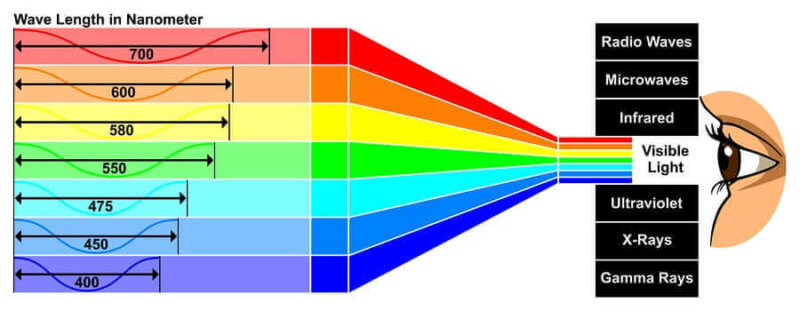
\includegraphics[scale=0.45]{colorimetria3}
            \caption{Lo spettro visibile}
        \end{figure}
        \newpage
        \subsubsection{Percezione del colore}
        Il colore nasce dalla luce. La luce che colpisce un oggetto viene parzialmente assorbita a
        seconda del materiale che lo compone. La parte non assorbita viene riflessa e trasmessa ai recettori cromatici
        all’interno dell’occhio umano. Questi ultimi trasformano la luce assorbita in impulsi che
        percorrono le vie nervose fino a raggiungere il cervello, dove vengono interpretati: nasce così
        un’impressione cromatica. \\
        Dal punto di vista prettamente biologico il colore si genera pertanto
        nell’occhio dell’osservatore e costituisce un’impressione sensoriale.
        Proprio perché nella percezione del colore vengono coinvolte componenti biologiche, ciascun individuo percepisce il colore in modo
        differente.
        Perfino la stessa persona può percepire differentemente il colore in momenti diversi ed in base
        allo stato d’animo. È quindi molto complesso definire in maniera oggettiva un colore.

        \begin{figure}[h]
            \centering
            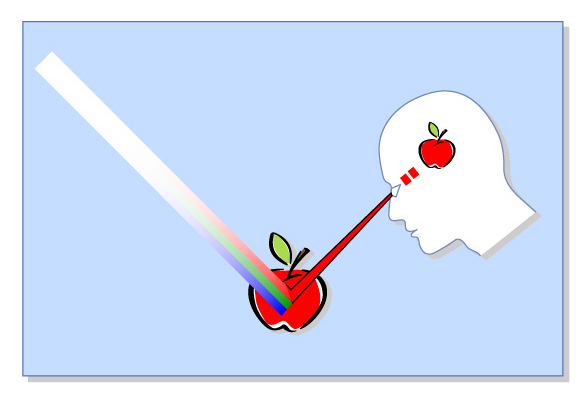
\includegraphics[scale=0.8]{colorimetria1}
            \caption{Percezione del colore}
        \end{figure}
        \newpage
        \subsection{Spazio colore}
        Per rappresentare in maniera rigorosa i colori, sono nati gli spazi colore. Ognuno di essi si basa su alcuni parametri
        e facendoli variare si riesce a rappresentare un numero più o meno grande di colori. Esistono numerosi spazi colore
        che, in base alle loro peculiarità, si prestano meglio ad uno specifico utilizzo piuttosto che ad un altro.
       
        \subsubsection{Modello CIE XYZ}
        Un importante spazio colore è il modello CIE XYZ che rappresenta tutti i colori caratterizzati da tre parametri: luminosità, tinta e purezza, rappresentati attraverso un solido. 
        Del solido viene solitamente rappresentata soltanto la sezione secondo il piano XY, in cui X ed Y indicano la cromaticità (tinta e purezza) mentre la luminosità non viene rappresentata.
        \begin{figure}[h]
            \centering
            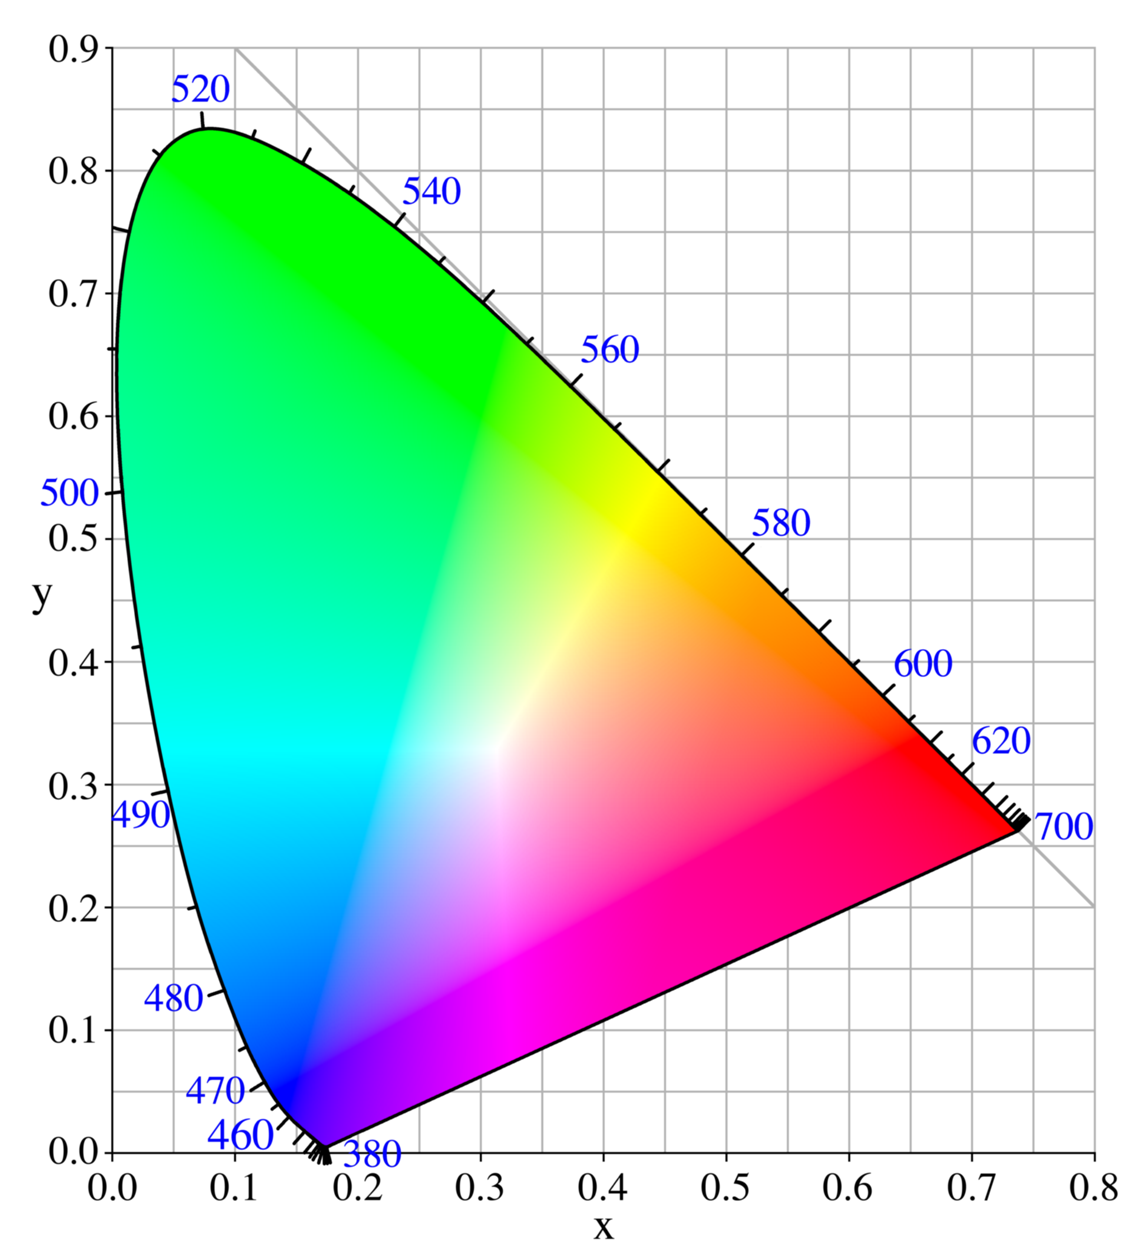
\includegraphics[scale=0.2]{CIEXYZ.png}
            \caption{Spazio colore CIE XYZ}
        \end{figure}
        \\Questo spazio colore si basa sui valori di tristimolo, cioè dei parametri che definiscono il modo in cui l'essere umano percepisce i colori. 
        I valori tristimolo di un colore con una distribuzione di potenza spettrale $I(\lambda)$  sono date in termini di un osservatore standard da:
        \\[0.2in]
            $\textbf{X}=\bigint_0^\infty I(\lambda)\,\overline{x}(\lambda)\,d\lambda$;
            $\textbf{Y}=\bigint_0^\infty I(\lambda)\,\overline{y}(\lambda)\,d\lambda$;
            $\textbf{Z}=\bigint_0^\infty I(\lambda)\,\overline{z}(\lambda)\,d\lambda$.
      
        
    
        \newpage

        \subsubsection{Modello CIE L*a*b*}
        A partire dallo spazio colore CIE XYZ si è poi sviluppato il modello CIE L*a*b*. Esso è un modello tridimensionale che si sviluppa lungo tre assi ortogonali. Due assi sul piano orizzontale riguardano la cromaticità: l'asse \textbf{a} si estende dal verde (-a) al rosso (+a)
        e l'asse \textbf{b} dal blu (-b) al giallo (+b); vi è poi un asse verticale che riguarda la luminosità o luminanza \textbf{L} che varia dal basso verso l'alto.
        Questo particolare spazio colore include tutti i colori percepibili dall'occhio umano e quindi anche tutto il gamut degli spazi RGB e CMYK ed è indipendente dal dispositivo che li rappresenta.
        Essendo quindi molto più simile al modo in cui l'essere umano riesce a percepire i colori, questo spazio colore si presta particolarmente bene agli scopi di questa ricerca.
        \begin{figure}[h]
            \centering
            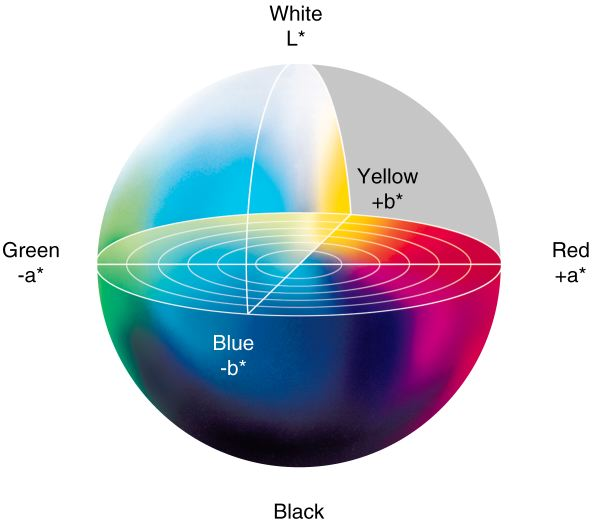
\includegraphics[scale=0.6]{CIELAB.jpg}
            \caption{Spazio colore CIE L*a*b*}
        \end{figure}

    \newpage
    \subsection{Risoluzione e compressione}
    La risoluzione di un'immagine corrisponde al numero di pixel per pollice che contiene, indicata con il termine in dpi (punti per pollice). 
    Un maggior numero di dpi si traduce in una maggiore quantità di informazioni e quindi in una qualità dell'immagine superiore. 
    Ovviamente, maggiore è il numero di informazioni che un'immagine contiene, maggiore sarà il peso del file. 
    Per questa ragione, sono state sviluppate alcune tecniche di compressione tra cui quella JPEG. Questa tecnica stabilisce due metodi di compressione di base,
    uno basato sull'uso della trasformata discreta del coseno, con compressione di tipo "lossy" e cioè con perdita di informazione, e l'altro sull'uso di un metodo predittivo
    con compressione di tipo lossless, cioè senza perdita di informazione. La perdita di informazioni durante la compressione può compromettere drasticamente la qualità dell'immagine.
    \begin{figure}[h]
        \centering
        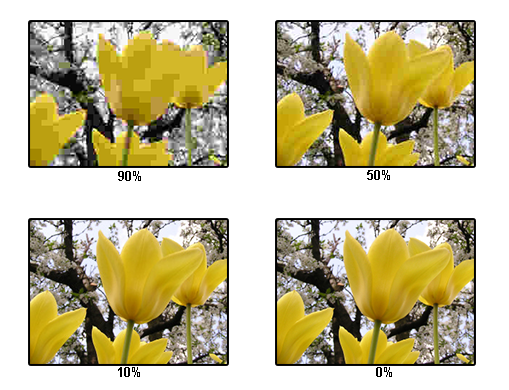
\includegraphics[scale=0.7]{jpeg.png}
        \caption{Esempio di compressione JPEG}
    \end{figure}
    \newpage
    \subsubsection{Esempi di risoluzione}
    Ai fini della nostra ricerca, sono state prese in considerazione 5 risoluzioni diverse. Ad ogni risoluzione
    è associata una coppia di valori numerici rappresentativi della larghezza e dell'altezza dell'immagine:
    \begin{itemize}
        \item 4K $\rightarrow$ 3840x2160;
        \item 3K $\rightarrow$ 3000x2000;
        \item 1080p $\rightarrow$ 2048x1080;
        \item 720p $\rightarrow$ 1280x720;
        \item 480p $\rightarrow$ 544x480;
    \end{itemize}
    Il prodotto di questi valori rappresenta il numero di pixel presenti in un'immagine ad una data risoluzione.
    Ad esempio, a 4K avremo:
    $$3840*2160 = 8.294.400$$
    mentre a 480p il numero di pixel sarà:
    $$544*480 = 261.120$$
    Quindi un'immagine a 4K userà un numero di pixel decisamente superiore rispetto ad una a 480p e questo le consentirà
    di rappresentare l'immagine con un numero di dettagli superiore e quindi ad una qualità maggiore.
    \newpage
    \section {Reti Neurali}
    \subsection {Reti neurali e cervello umano}
    Le reti neurali artificiali sono nate per emulare attività tipiche del
    cervello umano. Risultano quindi molto utili per risolvere problemi di riconoscimento delle immagini o del linguaggio umano.
    Per riuscire ad emulare questi comportamenti ci si è quindi ispirati al funzionamento del cervello umano.
    Nel sistema nervoso esistono miliardi di neuroni. Un
    neurone è formato da un corpo cellulare e da molti prolungamenti
    ramificati, detti dendriti, attraverso i quali il neurone riceve segnali
    elettrici da altri neuroni. Ogni neurone ha anche un prolungamento
    filamentoso chiamato assone. All’estremità l’assone si ramifica formando terminali
    attraverso i quali i segnali elettrici vengono trasmessi ad altre cellule.
    Tra un terminale di un assone e la cellula ricevente esiste uno spazio. I segnali superano questo spazio per
    mezzo di sostanze chimiche dette neurotrasmettitori. Il punto di
    connessione tra terminale e dendrite è detto sinapsi. 
    Un neurone si “attiva”, cioè trasmette un impulso elettrico lungo il suo
    assone quando si verifica una differenza di potenziale elettrico tra l’interno
    e l’esterno della cellula. L’impulso elettrico provoca la liberazione di un
    neurotrasmettitore dai terminali dell’assone, che a loro volta possono influenzare altri neuroni. 
        
    \begin{figure}[h]
        \centering
        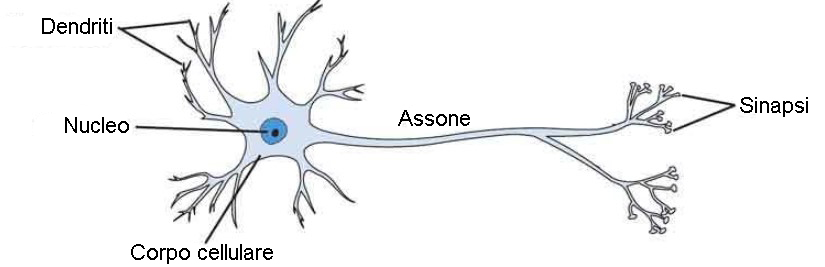
\includegraphics[scale=0.7]{cervello.jpg}
        \caption{Neurone biologico}
    \end{figure}

    \subsubsection{Dal neurone biologico a quello artificiale}
    
    Per riprodurre artificialmente il cervello umano occorre realizzare
    una rete di elementi molto semplici in grado di imparare e generalizzare.
    Tipicamente, il neurone artificiale ha molti ingressi ed una sola uscita.
    Per determinare la conducibilità e quindi l'importanza del canale di ingresso, ogni neurone ha associato un peso. 
    L’attivazione del neurone è una funzione della somma pesata degli ingressi.\\[1in]
    Il metodo più usato per addestrare una rete neurale consiste nel presentare
    in ingresso alla rete un insieme di esempi (training set). 
    La risposta fornita dalla rete per ogni esempio viene confrontata con la risposta desiderata, si
    valuta la differenza (errore) fra le due e, in base a tale differenza, si
    modificano i pesi cercando di ottenere il risultato desiderato.
    \begin{figure}[h]
        \centering
        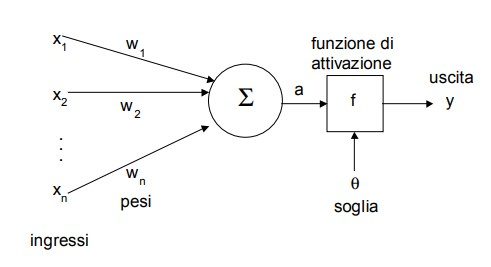
\includegraphics{neurone.jpg}
        \caption{Modello di neurone}
    \end{figure}
    \\In generale si hanno quindi $n$ ingressi $x_1, …, x_n$, a ciascuno dei quali è associato un peso. 
    I pesi $w_i$ sono numeri reali che riproducono l'amplificazione o lo smorzamento subito dal segnale nella comunicazione fra neuroni. Se $w_i > 0$, il canale è detto eccitatorio, se $w_i < 0$, il canale è inibitorio. 
    Il valore assoluto di un peso rappresenta la forza della connessione. 
    L’uscita, cioè il segnale con cui il neurone trasmette la sua attività
    all’esterno, è calcolata applicando la funzione di attivazione alla somma
    pesata degli ingressi:
    
    $$y = f(\sum_{i=1}^{n}w_i x_i)$$

    \subsection{Perceptron}
    Un semplice esempio di rete neurale è il perceptron. Un perceptron è una rete neurale ad un singolo livello che si dimostra molto utile nei problemi di classificazione.
    In generale è composto da una serie $x_1, ..., x_n$ di input a cui sono associati dei pesi $w_1, ..., w_n$. 
    Vi è poi una funzione che si occupa di sommare i prodotti dei valori di input e dei rispettivi pesi. 
    Il risultato passa infine per una funzione di attivazione che genera l'output.

    \newpage
    \subsubsection{Addestramento del perceptron}
    Per addestrare un perceptron bisogna realizzare un dataset adeguato per il problema che si vuole risolvere. 
    Dopo aver predisposto il dataset è necessario seguire i seguenti passi:
    \begin{enumerate}
        \item si inizializzano i pesi $w_i$ con valori casuali;
        \item si presenta alla rete un ingresso $x_k$, si confronta col $t_k$ desiderato in uscita;
        \item si calcola la risposta $y_k$ della rete e si aggiornano i pesi mediante la delta rule con l'obiettivo di ridurre l'errore;
        \item si ripete il ciclo dal passo 2, finché la risposta della rete non risulta soddisfacente.
    \end{enumerate}

    In particolare la delta rule è una regola usata per modificare i valori dei pesi di un neurone andando alla ricerca di quelli più adeguati.
    Dati $t$ ed $y$, rispettivamente l'uscita desiderata e l'uscita neurale, l'errore $\delta$ è dato da:
    $$ \delta = t-y.$$
    Fissato un numero reale $\eta$, compreso tra 0 e 1, detto learning rate, la delta rule stabilisce che la variazione del generico peso $\Delta w_i$ è:
    $$ \Delta w_i = \eta \delta x_i.$$

    Dopo l’addestramento la rete viene testata controllandone il comportamento su un insieme di dati, detto test set, non utilizzati durante la fase di training. La fase di test ha quindi lo scopo 
    di valutare la capacità di generalizzazione della rete neurale.

  
    \newpage
    \section{Svolgimento}

    \subsection{Creazione del dataset}
    Per poter realizzare la rete è necessario creare un dataset significativo affinché questa possa essere addestrata e testata. 
    Per fare ciò sono state prese in considerazione 40 immagini, nello spazio colore L*a*b*, ad una risoluzione di 4K, sulle quali sono state successivamente fatte delle elaborazioni.

    In particolare le elaborazioni sono state:
    \begin{enumerate}
        \item Per ogni immagine nel dataset iniziale è stata generata un'immagine ad una risoluzione minore o uguale (4K, 3K, 1080p, 720p, 480p).
        \item Per ogni immagine generata al punto 1 sono stati applicati tre filtri cromatici ciascuno a tre intensità diverse.
    \end{enumerate}
    Due dei filtri utilizzati coinvolgono indistintamente tutte le zone dell'immagine, mentre il terzo filtro altera solo le zone di una specifica tonalità di colore, in questo caso quelle del blu, in quanto maggiormente presente nel nostro dataset e le cui variazioni sono più complesse da individuare. 
    Questo procedimento ha così generato 2000 immagini, utilizzabili per addestrare e testare la rete.
    
    \begin{figure}[h]
        \centering
        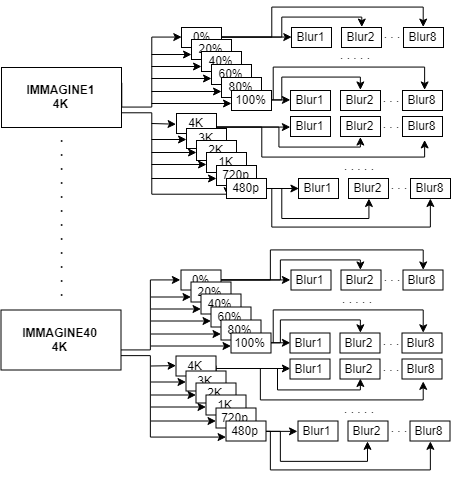
\includegraphics[scale=0.55]{generazione.png}
        \caption{Generazione del dataset}
    \end{figure}
    \newpage



    \subsubsection{Codice C++}
    Per ottenere il risultato, precedentemente descritto nel paragrafo 4.1, è stato sviluppato un programma in C++ sfruttando la libreria OpenCV.
    Per ogni immagine in una specifica directory, vengono generate le immagini a risoluzioni più basse e, per ognuna di queste, vengono applicati i filtri:
    \begin{lstlisting}[language=C++]
        for (dimension resolution : resolutions){
				Size size(resolution.height, resolution.width);
				Mat resizedImage;
				resize(imageOriginal, resizedImage, size);
				string newPath = basePath + "resized/" + resolution.name + "/" + fileName + ".tif";

				if (resolution.name.compare("4K") == 0) 
					copyFile(filePath, newPath);
				else
					imwrite(newPath, resizedImage);
            for (int intensityF1 = 6, double intensityF2 = 1.1, int intensityF3 = 5; intensityF1 <= 56, intensityF2 <= 1.5; intensityF3 <= 15; intensityF1 += 25, intensityF2 += 0.2, intensityF3 += 5) 
            {    
                Mat imageFiltered = applyFilter(newPath, 1, intensityF1);
                string newPathFiltered = basePath + "resized/" + resolution.name + "/filters/" + explode(fileName, '_')[0] + "_B" + to_string(nameCounter) + ".tif";
                imwrite(newPathFiltered, imageFiltered);
                
                imageFiltered = applyFilter(newPath, 2, intensityF2);
                newPathFiltered = basePath + "resized/" + resolution.name + "/filters/" + explode(fileName, '_')[0] + "_B" + to_string(nameCounter+3) + ".tif";
                imwrite(newPathFiltered, imageFiltered);

                imageFiltered = applyFilter(newPath, 3, intensityF3);
                newPathFiltered = basePath + "resized/" + resolution.name + "/filters/" + explode(fileName, '_')[0] + "_B" + to_string(nameCounter+6) + ".tif";
                imwrite(newPathFiltered, imageFiltered);

                nameCounter++;
            }
        }
    \end{lstlisting}

    \newpage
    \subsubsection{Esempi di applicazione dei filtri}
    Di seguito vengono riportati alcuni esempi di immagini generate con il precedente procedimento le cui differenze sono facilmente percepibili ad occhio nudo.
    \begin{figure}[h]
        \centering
        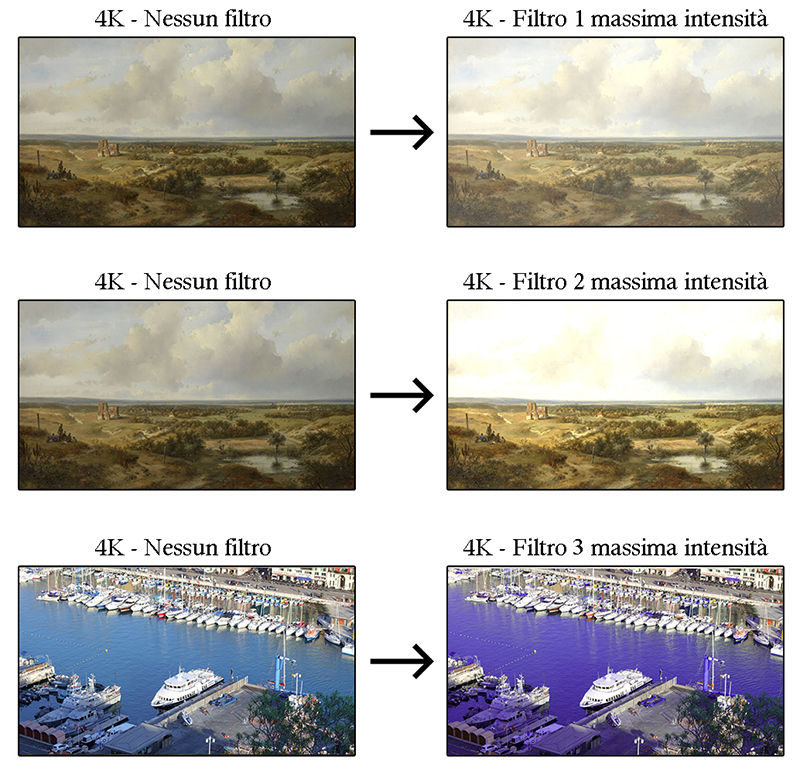
\includegraphics[scale=0.45]{filtri}
        \caption{Esempi di applicazione dei filtri}
    \end{figure}


    \newpage
    
    \subsection{Feature Extraction}
    Per addestrare la rete si è deciso di usare un tipo di addestramento detto "supervisionato". 
    L'addestramento supervisionato è una tecnica di apprendimento automatico che mira a istruire una rete in modo da consentirgli di elaborare automaticamente previsioni sui valori di uscita di un sistema rispetto 
    ad un input, sulla base di una serie di esempi ideali costituiti da coppie di input e di output, che gli vengono inizialmente forniti. L'estrazione delle informazioni dal dataset da fornire come input alla rete viene detta Feature Extraction.
    
    \subsubsection{Preparazione degli input e degli output}
    Affinché si possa procedere con l'addestramento, è necessario fornire alla rete dei dati, in grado di rappresentare
    tutte le immagini da confrontare (input). Dobbiamo inoltre fornire delle valutazioni effettuate da un osservatore umano (output), che indichino la somiglianza tra le varie coppie di immagini da confrontare. 
    Studiando questi dati la rete sarà in grado di emulare il comportamento umano nell'identificazione delle differenze percettive tra due immagini.

    \subsubsection{Estrazione dei dati dalle immagini}
    I dati di input vengono estratti dalle immagini nel nostro dataset, illustrato nel paragrafo 4.1. In particolare, questi dati faranno riferimento a zone delle immagini sufficientemente grandi da poter permettere alla rete di comprenderne
    non solo il colore, ma anche la struttura, distinguendone forme e dettagli generali. Per fare ciò, tutte le immagini sono
    state suddivise in 9 zone di dimensione uguale e per ognuna di esse sono stati calcolati i valori di media e varianza (dette feature). Questo procedimento
    viene effettuato per ognuno dei 3 canali (L, a, b).
    Per la media è stata usata la funzione mean() della libreria OpenCV, mentre per la varianza è stata implementata una funzione apposita: 
    \begin{lstlisting}[language=C++]
    double variance(Mat & m, int i, int j, int block_height, int block_width)
    {
        double variance = 0;
        Mat m_tmp = m(Range(i, i + block_height), Range(j, j + block_width)); 
        Mat m_squared(block_height, block_width, CV_64F); 
        
        multiply(m_tmp, m_tmp, m_squared);
        
        double avg = mean(m_tmp)[0]; 	
        double avg_2 = mean(m_squared)[0]; 	
        var = sqrt(avg_2 - avg * avg);
        return variance;
    }
    \end{lstlisting}
    Media e varianza sono tipicamente utilizzati in colorimetria proprio per scopi simili, come ad esempio, nel calcolo dell'SSIM.

    La rete dovrà avere in ingresso la lista dei valori di ogni immagine originale, associata ad ogni sua immagine filtrata. 
    Dopo aver calcolato i valori, questi vengono inseriti in una matrice di dimensione 1800x108, dove 1800 è il numero di coppie ($Im_i$, $F_j(Im_i, in)$)
    con $Im_i$ immagine $i$-esima, $F_j$ funzione filtro $j$-esima e $in$ intensità del filtro, mentre 108 è il numero di feature calcolate per ogni coppia.
    
    In particolare, date $X$ ed $Y$ rispettivamente immagine originale e filtrata, $n$ numero di zone su cui sono suddivise le immagini,
    una riga della matrice contiene: 
    \begin{itemize}
        \item ${\mu_x}_i(C)$: media di ogni zona dell'immagine $X$ nei 3 canali;
        \item ${\mu_y}_i(C)$:  media di ogni zona dell'immagine $Y$ nei 3 canali;
        \item ${\sigma^2_x}_i(C)$: varianza di ogni zona dell'immagine $X$ nei 3 canali;
        \item ${\sigma^2_y}_i(C)$: varianza di ogni zona dell'immagine $Y$ nei 3 canali;
    \end{itemize}
    con $i \in (1,n)$ e $C \in (L, a, b)$.
    \\Le feature sono quindi: 3 canali * 9 finestre * 4 valori = 108, per riga.
    La matrice di questi valori rappresenterà quindi l'input della nostra rete ed ogni sua riga è detta sample.
    \newpage
    \subsubsection{Codice C++}
    Per estrapolare queste fetures è stata realizzata la seguente funzione C++:
    \begin{lstlisting}[language=C++]
        for (int k = 0; k < nbBlockPerHeight; k++){
            for (int l = 0; l < nbBlockPerWidth; l++)
            {
                int m = k * block_height;
                int n = l * block_width;
                // Media canale b
                double avg_ob = mean(img_original[0](Range(k, k + block_height), Range(l, l + block_width)))[0];
                double avg_cb = mean(img_filtered[0](Range(k, k + block_height), Range(l, l + block_width)))[0];
                values.push_back(avg_ob);
                values.push_back(avg_cb);
                // Media canale a
                double avg_oa = mean(img_original[1](Range(k, k + block_height), Range(l, l + block_width)))[0];
                double avg_ca = mean(img_filtered[1](Range(k, k + block_height), Range(l, l + block_width)))[0];
                values.push_back(avg_oa);
                values.push_back(avg_ca);
                // Media canale L
                double avg_oL = mean(img_original[2](Range(k, k + block_height), Range(l, l + block_width)))[0];
                double avg_cL = mean(img_filtered[2](Range(k, k + block_height), Range(l, l + block_width)))[0];
                values.push_back(avg_oL);
                values.push_back(avg_cL);
                // Varianza canale b
                double sigma_oa = variance(img_original[2], m, n, block_height, block_width);
                double sigma_ca = variance(img_filtered[2], m, n, block_height, block_width);
                values.push_back(sigma_oa);
                values.push_back(sigma_ca);
                // Varianza canale a
                double sigma_ob = variance(img_original[1], m, n, block_height, block_width);
                double sigma_cb = variance(img_filtered[1], m, n, block_height, block_width);
                values.push_back(sigma_ob);
                values.push_back(sigma_cb);
                // Varianza canale L
                double sigma_oL = variance(img_original[0], m, n, block_height, block_width);
                double sigma_cL = variance(img_filtered[0], m, n, block_height, block_width);
                values.push_back(sigma_oL);
                values.push_back(sigma_cL);
            }
        }
    \end{lstlisting}   
    \subsubsection{Preparazione degli output}
    Affinché la rete possa esprimere un giudizio di somiglianza relativamente a una coppia di immagini da confrontare,
    si sono considerati 5 livelli crescenti di affinità: Low(L), Medium-Low(ML), Medium(M), Medium-High(MH), Hight(H).
    La rete è quindi un classificatore a cinque classi. Questi sono indicativi di quanto due immagini siano simili tra loro.
    Sono state quindi analizzate 1800 coppie di immagini (40 immagini * 9 immagini filtrate * 5 risoluzioni), e ad ognuna di queste
    è stato assegnato un giudizio in questa scala.
    Così come un essere umano riesce ad individuarne le differenze guardando una coppia di immagini, la rete neurale si comporterà esattamente allo stesso modo ma 
    guardando alle immagini come un insieme di caratteristiche espresse da valori numerici.
    Guardando i valori rappresentativi di una coppia di immagini, la rete cercherà di estrapolare un giudizio basandosi sulla sua esperienza pregressa.
    Questa esperienza le viene fornita mostrandole degli esempi, forniti da un osservatore umano che dovrà effettuare tutti i confronti tra le varie coppie di immagini e dare una sua valutazione.
    Quando la rete sarà giunta ad un responso, dovrà comunicare all'esterno il suo risultato. Per farlo utilizzerà i neuroni di output, attivando quello corrispondente al giudizio che ha ottenuto.
    I neuroni di uscita saranno quindi 5, uno per ogni giudizio possibile, e il valore di uscita della rete sarà:
    \begin{itemize}
        \item {0,0,0,0,1} $\rightarrow$ L 
        \item {0,0,0,1,0} $\rightarrow$ ML
        \item {0,0,1,0,0} $\rightarrow$ M
        \item {0,1,0,0,0} $\rightarrow$ MH
        \item {1,0,0,0,0} $\rightarrow$ H
    \end{itemize}
    Dove con 1 si indica il neurone attivo e con 0 il neurone non attivo.
    \newpage
    \subsubsection{Esempio di risposta della rete}
    Spieghiamo ciò che si vuole ottenere dalla rete neurale attraverso un esempio. Si considerino due immagini, una originale ed una a cui è stato applicato il primo filtro alla massima intensità.
    Da esse sono state estratte le feature, come visto nel paragrafo 4.2.2, che vengono poi passate in input ad una rete addestrata.
    Passando attraverso una serie di "livelli nascosti", che la rete crea per effettuare le elaborazioni necessarie all'ottenimento dell'output,
    la rete si accorge che le due immagini sono percettivamente molto diverse tra loro. Procede quindi attivando l'ultimo neurone di uscita.
    \begin{figure}[h]
        \centering
        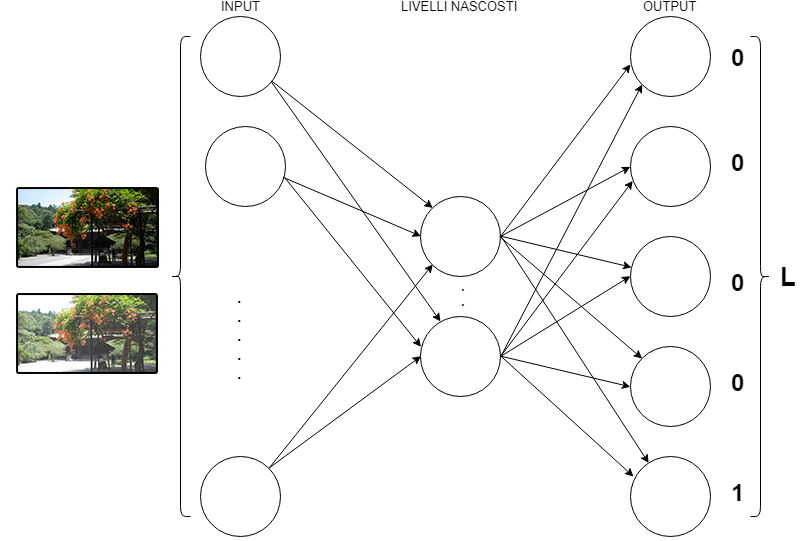
\includegraphics[scale=0.4]{reteneurale}
        \caption{Esempio di risposta della rete}
    \end{figure}

    \newpage
    \subsubsection{Esempi di valutazioni da parte dell'osservatore}
    L'osservatore umano, compirà lo stesso procedimento ma assegnando un valore simbolico ad ogni coppia di immagini, come illustrato nel paragrafo 4.2.4.
    Di seguito vengono riportati alcuni esempi di valutazioni effettuate dall'osservatore.
    \begin{figure}[h]
        \centering
        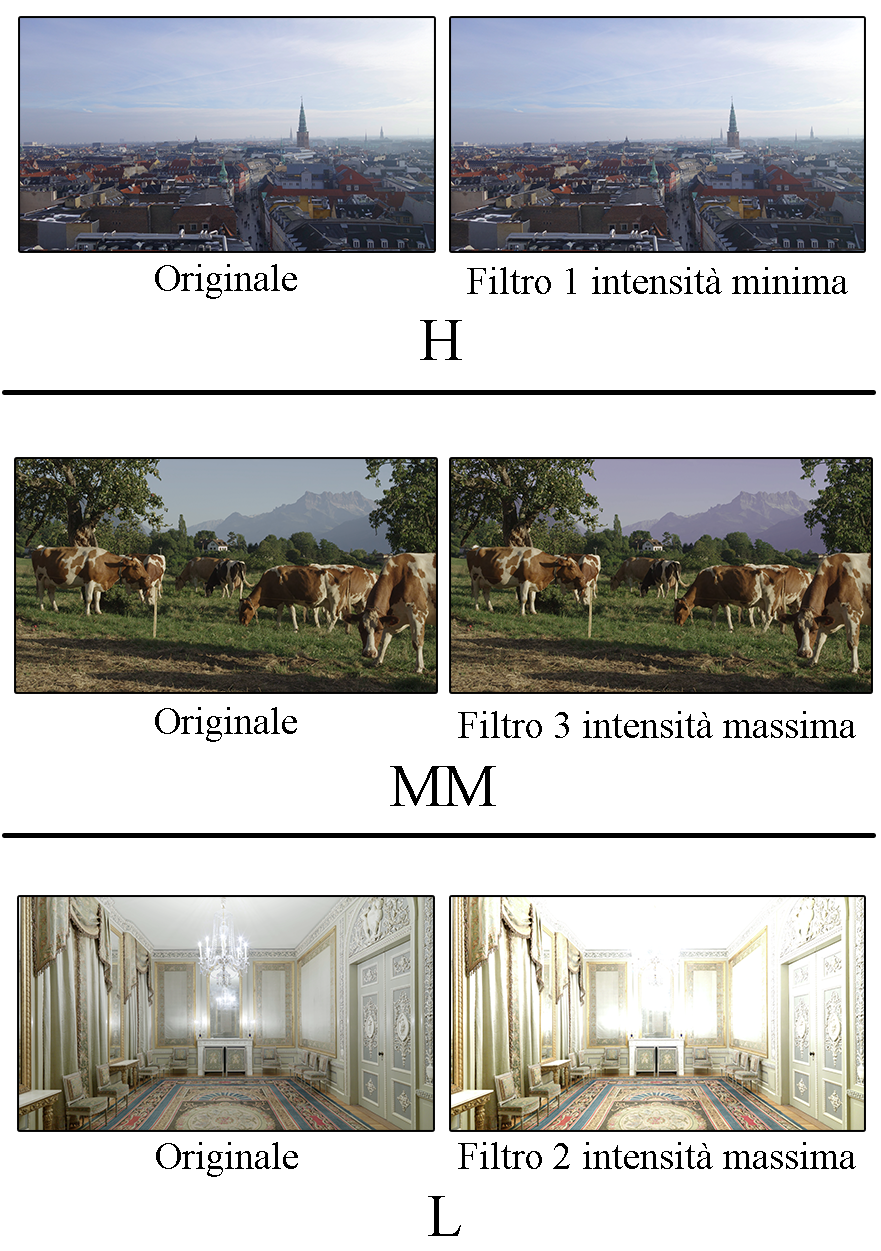
\includegraphics[scale=0.3]{confronto.png}
        \caption{Esempi di risposta dell'osservatore umano}
    \end{figure}
    \newpage
    \subsection{Considerazioni preliminari}
    Prima di procedere con l'addestramento della rete, analizziamo i dati ottenuti nei precedenti paragrafi. 
    \subsubsection{Analisi dei giudizi dell'osservatore}
    Prendendo in considerazione tutte le 1800 coppie di immagini originali e filtrate e associandole ai rispettivi giudizi dati
    dall'osservatore nel paragrafo 4.2.4, si nota una tendente accentuazione delle differenze cromatiche, al diminuire della risoluzione.
    In particolare, prendendo come esempio il giudizio dato ad una coppia di immagini a 4K e confrontandolo con quello della stessa coppia a risoluzioni inferiori, per tutte le possibili coppie nel dataset,
    si ottengono i seguenti risultati:
    \begin{figure}[h]
        \centering
        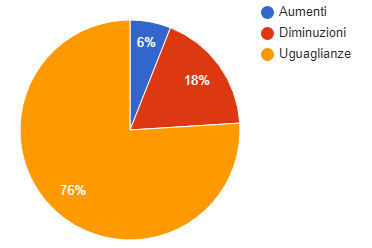
\includegraphics{chart1}
        \caption{"Variazione della percezione umana"}
    \end{figure}
    \\Come si evince dal grafico, all'abbassarsi della risoluzione, le differenze percettive tra le immagini rimangono nella maggioranza dei casi invariate e tendono ad essere accentuate, causando così
    una valutazione più bassa dell'indice di similarità. Ciò accade nel 94\% dei casi presi in considerazione.
    \newpage
    \subsubsection{Calcolo del Lab-SSIM}
    Per avvalorare questa tesi ed evitare che questo comportamento possa essere riconducibile solo alla percezione dell'osservatore umano preso in considerazione, si è deciso
    di effettuare lo stesso procedimento considerando però un indice matematico capace di esprimere le differenze percettive tra due immagini L*a*b*, il Lab-SSIM.
    Questo indice è diverso dall'SSIM tradizionale e consiste nel calcolare, i valori di luminanza dei canali a e b, di contrasto e di struttura del canale L e fare la media tra tutti questi valori.
    \begin{figure}[h]
        \centering
        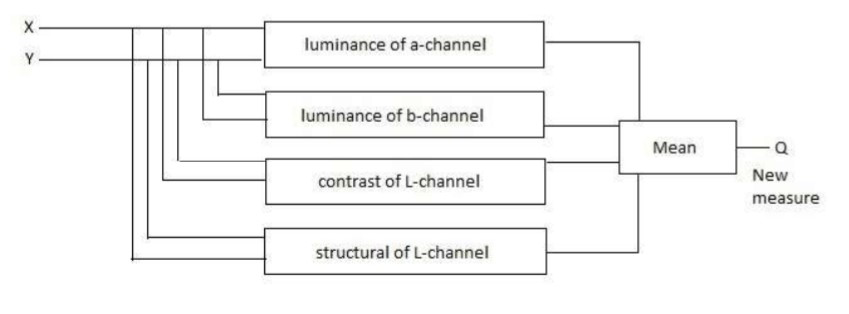
\includegraphics[scale=0.7]{labssim.png}
        \caption{Lab-SSIM}
    \end{figure}

    Il Lab-SSIM si basa quindi su tre misurazioni di confronto tra i campioni di $x$ e $y$: luminanza $l$, contrasto $c$ e struttura $s$. Le singole funzioni di confronto sono:
    \begin{enumerate} 
        \item $l(x,y)=\frac{2\mu_x\mu_y + c_1}{\mu^2_x + \mu^2_y + c_1}$
        \item $c(x,y)=\frac{2\sigma_x\sigma_y + c_2}{\sigma^2_x + \sigma^2_y + c_2}$
        \item $s(x,y)=\frac{\sigma_{xy} + c_3}{\sigma_x \sigma_y + c_3}$
    \end{enumerate}
    in cui si hanno:
    \begin{itemize} 
        \item $\mu_x$ e $\mu_y$ sono, rispettivamente, la media di $x$ e $y$;
        \item $\sigma_x^2$ e $\sigma_y^2$ sono, rispettivamente, la varianza di $x$ e $y$;
        \item $\sigma_{xy}$ è la covarianza di $x$ e $y$;
        \item $c_1=(k_1L)^2$, $c_2=(k_2L)^2$ sono due variabili per stabilizzare la divisione con il denominatore inadatto;
        \item $c_3$ è una costante pari a $c_2 / 2$.
        \item $k_1=0.01$ e $k_2=0.03$ sono costanti predefinite.
   \end{itemize}
   \newpage
    
    \subsubsection{Analisi dei risultati ottenuti con il Lab-SSIM}
    Dopo aver calcolato il Lab-SSIM per tutte le coppie di immagini da confrontare, si passa ad analizzare i risultati, cercando di capire
    se, abbassando la risoluzione, le differenze continuano ad essere visibili. Si fanno quindi le stesse considerazioni del paragrafo 4.3, ma questa volta
    considereremo come giudizio l'indice matematico e non il giudizio dato dall'osservatore umano.
    \begin{figure}[h]
        \centering
        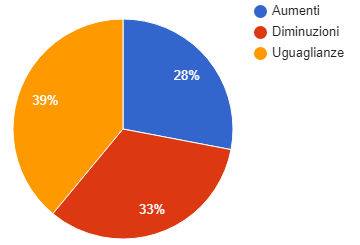
\includegraphics{chart2}
        \caption{Variazione del Lab-SSIM}
    \end{figure}
    \\In questo caso, i giudizi rimangono invariati o si abbassano nel 72\% dei casi. La tendenza sembra quindi essere confermata.    Da questi risultati si può già dedurre che all'abbassarsi della risoluzione, le differenze percettive non solo rimangono percepibili ma tendono addirittura ad accentuarsi.
    \newpage
    \subsection{Addestramento della rete}
    Adesso che siamo in possesso degli input e degli output da fornire alla rete, possiamo passare ad effettuare un primo addestramento.
    Considerando $x$ e $t$ rispettivamente l'insieme delle feature estratte dalle immagini e l'insieme dei giudizi dati dall'osservatore, si addestra la rete
    utilizzando il seguente codice Matlab:
    \begin{lstlisting}[language=Matlab]        
        % Funzione di training
        trainFcn = 'trainlm';  
        
        % Creazione della rete
        hiddenLayerSize = 10;
        net = patternnet(hiddenLayerSize, trainFcn);
        
        % Suddivisione del dataset in training, test e validation set
        net.divideFcn = 'dividerand'; 
        net.divideMode = 'sample'; 
        net.divideParam.trainRatio = 70/100;
        net.divideParam.valRatio = 10/100;
        net.divideParam.testRatio = 20/100;
        
        % Funzione per il calcolo delle performance e lista di grafici da generare
        net.performFcn = 'mse';  % mean squared error
        
        net.plotFcns = {'plotperform','plottrainstate','ploterrhist', ...
            'plotconfusion', 'plotroc'};
        
        % Addestramento della rete
        [net,tr] = train(net,x,t);
        
        % Test della rete e performance
        y = net(x);
        e = gsubtract(t,y);
        performance = perform(net,t,y)
        tind = vec2ind(t);
        yind = vec2ind(y);
        percentErrors = sum(tind ~= yind)/numel(tind);
    \end{lstlisting}
    Il dataset iniziale è stato diviso in 3 parti: Training Set, Validation Set e Test Set. Essi servono rispettivamente per addestrare, validare e testare la rete.
    In particolare, il Training Set serve per far capire alla rete quali risposte deve dare in base agli input che gli vengono forniti, il Validation Set serve per evitare il fenomeno dell'overfitting, mentre il Test Set serve per valutarne le performance alla fine dell'addestramento.
    \newpage
    \subsubsection{Valutazione delle prestazioni}
    Una volta completato l'addestramento, per valutarne le prestazioni, analizziamo la matrice di confusione, che mostra, sulla diagonale, quanti sample sono stati valutati correttamente:
    \begin{figure}[h]
        \centering
        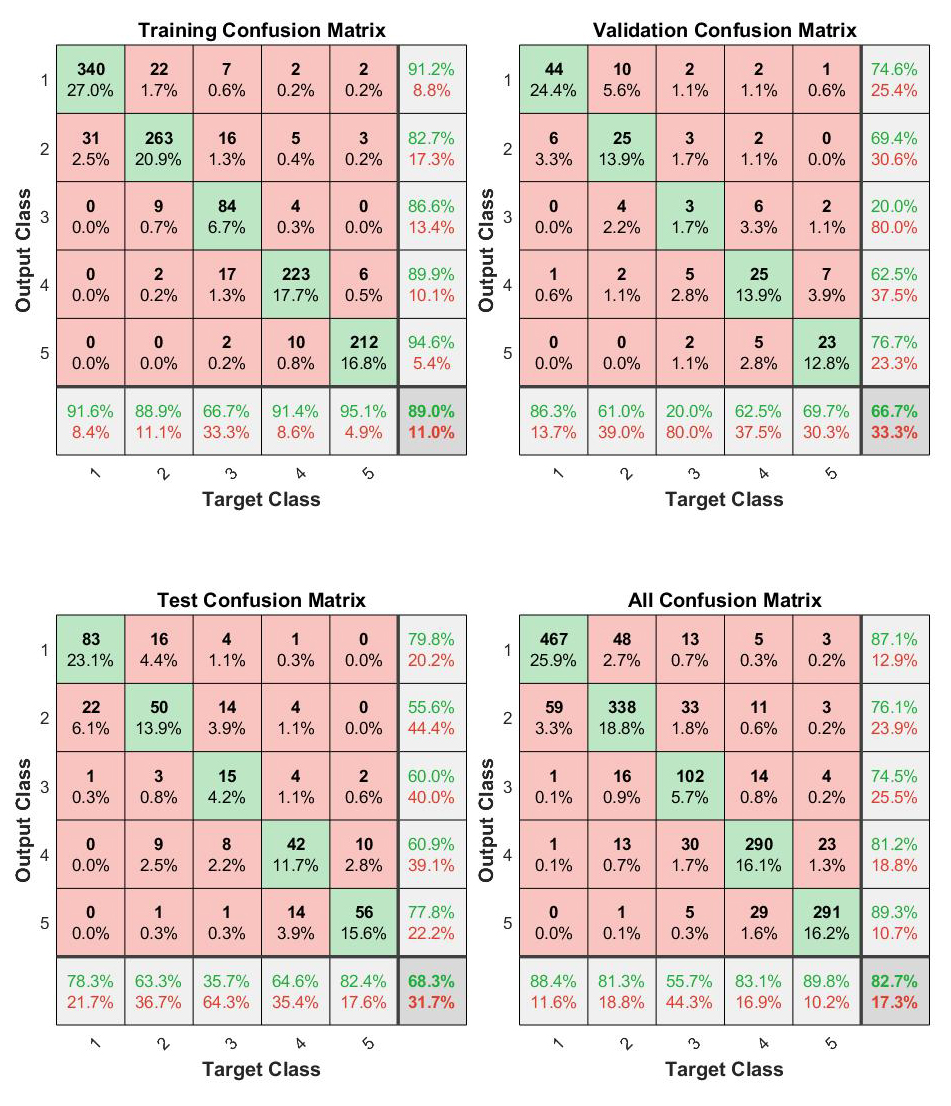
\includegraphics[scale=0.38]{confusion1}
        \caption{Matrice di confusione}
    \end{figure}
    \\Ciò che si evince è che l'accuratezza della rete è di poco inferiore al 70\%, precisamente 68.3\% sul Test set. 
    La precisione della rete è bassa, e può sicuramente essere migliorata. Idealmente, si vorrebbe ottenere che il 100\% dei giudizi fosse corretto e quindi
    la matrice dovrebbe avere valori soltanto sulla diagonale. In questo caso tuttavia, notiamo una buona precisione sulle valutazioni estreme (H ed L), ma una più scarsa capacità di giudizio delle coppie di immagini che hanno ricevuto una valutazione meno netta.
    Ciò può essere dovuto al fatto che le reti neurali necessitano di un grande numero di dati nel training set affinché possano essere addestrate in maniera corretta.
    Euristicamente, dato $x$ numero di feature in input alla rete, $t$ numero di neuroni di uscita, e $h$ numero di neuroni presenti nei livelli nascosti, il numero $n$ adeguato di esempi che devono essere presenti nel dataset deve essere:
    $$ n \geq ((x*h)+(t*h))*5.$$

    Nel nostro caso, le feature sono l'insieme di varianze e medie calcolate per tutte le coppie (108 feature), come descritto dettagliatamente nel paragrafo 4.2.2, i neuroni di output sono 5, mentre i neuroni nascosti sono fissati a 6 per ipotesi.
    Effettuando il calcolo di cui sopra, si ottiene: 
    $$ n \geq ((108*6)+(5*6))*5 = 3390.$$
    Quindi, per addestrare adeguatamente la nostra rete sarebbero necessari almeno 3390 esempi  di confronti tra coppie di immagini.
    Non disponendo di questi dati, ciò che possiamo fare è effettuare la feature selection, cioè l'identificazione delle feature maggiormente discriminanti tra le 108 ottenute durante la feature extraction.
    Riducendo il numero di feature in ingresso alla rete, anche il numero di esempi necessari sarà ridotto, potendo addestrare adeguatamente la rete anche con soli 1800 confronti.
    \subsection{Feature selection}
    Durante la feature selection, si applica un algoritmo in grado di identificare, tra le varie feature estratte durante la feature extraction, quelle con il maggiore potere discriminante.
    Conoscendo questo dato, è poi facile diminuire il numero di feature in ingresso alla rete, andando a selezionare solo quelle realmente necessarie. 
    Per effettuare la feature selection si comincia selezionando una feature dal dataset iniziale, essa sarà data in ingresso ad una rete che cercherà di calcolare il risultato di cui necessitiamo.
    Si osserva il risultato ottenuto e si sceglie la feature che, da sola, dà il più basso errore di classificazione. Si procede poi aggiungendo una feature e ritestando la rete con la coppia ottenuta. Si va avanti così aggiungendo di volta in volta una nuova feature ai test fino al soddisfacimento di un criterio.
    Questa tipologia di feature selection è detta forward sequential feature selection. Esiste anche quella backword in cui si parte dall'insieme totale delle feature e si procede eliminandone una ad ogni step.
    Alla fine di questo processo, si osservano i risultati della rete nei vari casi e si prendono le feature che hanno permesso di ottenere i risultati migliori.
    \newpage
    \subsubsection{Analisi dei risultati}
    Dopo oltre 300 iterazioni, la feature selection ha selezionato molteplici volte alcune particolari feature, considerandole quindi più importanti.
    Il seguente grafico mostra il numero di volte che una certa feature, appartenente al gruppo totale delle feature numerate da 1 a 108, è stata scelta durante la feature selection: 
    \begin{figure}[h]
        \centering
        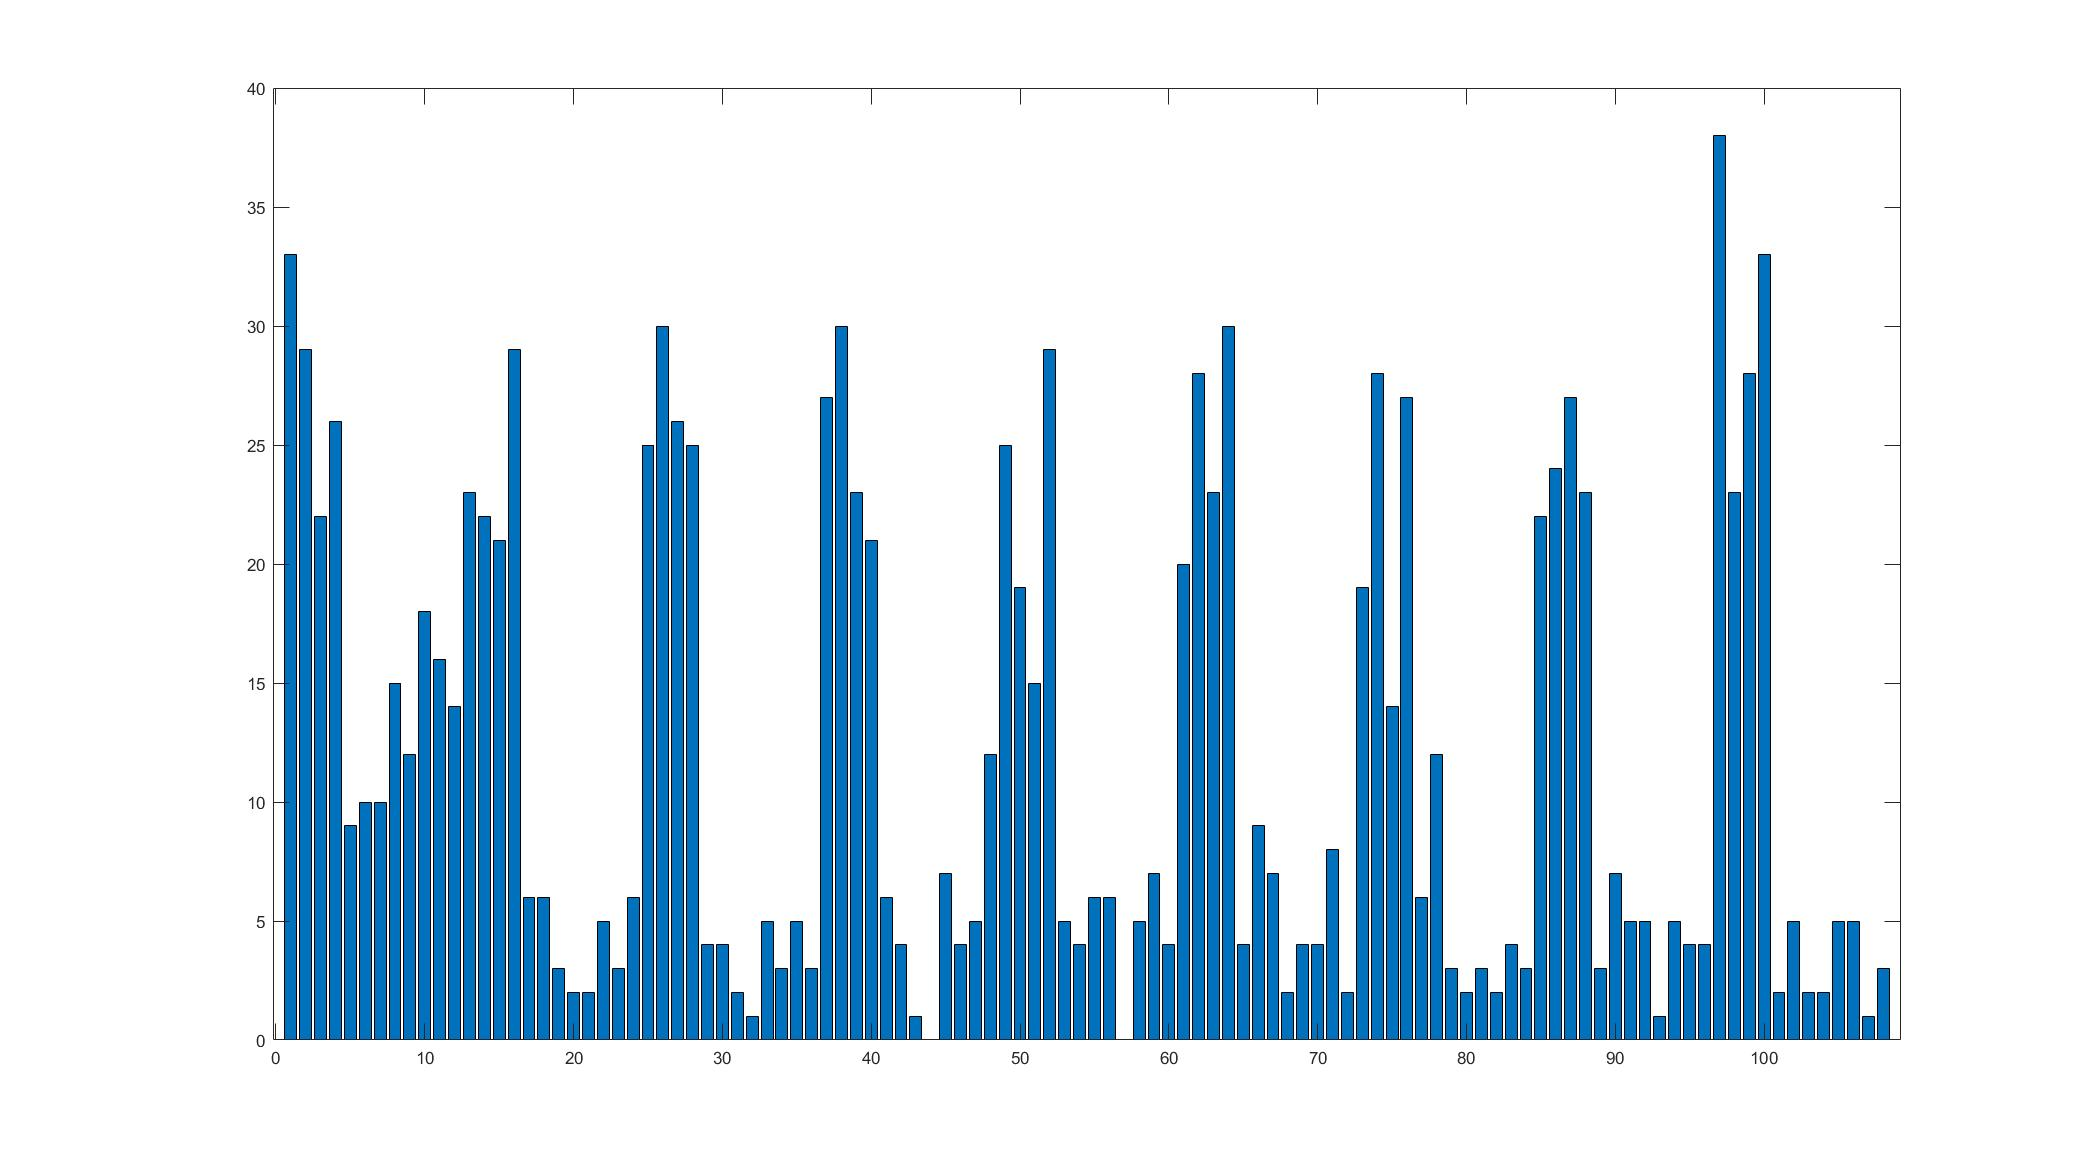
\includegraphics[scale=0.18]{featureselection}
        \caption{Risultati della Feature Selection}
    \end{figure}
    \\Analizzando il grafico si decide quindi di considerare per l'addestramento della rete soltanto le feature su cui sono presenti dei picchi evidenti di utilizzo. E' inoltre necessario assicurarsi di selezionare
    almeno una feature per ogni finestra, sia per l'immagine originale (x) che per quella a cui è stato applicato il filtro(y). Vengono quindi considerate le seguenti feature:
    Mx1(L), My1(L), Sx2(L), Sy2(L), Sx3(L), My3(L), Mx4(L), My4(L), Mx5(L), Sy5(L), Sx6(L), Sy6(L), My7(L), Sx7(L), Sx8(L), Sy8(L), My9(L), Sx9(L).\\
    In questo modo siamo riusciti ad ottenere una diminuizione sostanziale delle feature in ingresso alla rete, passando da 108 a 18.
    \newpage
    \subsubsection{Undersampling e oversampling}
    Un'ulteriore causa della scarsa precisione della rete può essere lo sbilanciamento del dataset. E' infatti molto probabile che, durante l'assegnamento dei giudizi da parte dell'osservatore umano, 
    una certa classe di risultati sia stata usata più volte rispetto ad un'altra. Si procede quindi calcolando le occorrenze dei vari giudizi dati dall'osservatore:
    \begin{itemize}
        \item H: 528
        \item MH: 416
        \item M: 183
        \item ML: 349
        \item L: 324
    \end{itemize}
    I risultati evidenziano un palese sbilanciamento causato da un eccessivo numero di H e un non sufficiente numero di M.
    Per riequilibrare la situazione si effettua l'undersampling, cioè la diminuizione dei sample, di H e l'oversampling, cioè la duplicazione dei sample, di M.
    \begin{itemize}
        \item H: 428
        \item MH: 416
        \item M: 366
        \item ML: 349
        \item L: 324
    \end{itemize}
    A seguito di questa elaborazione, il dataset è bilanciato e contiene un totale di 1883 sample.
    In questo modo la rete potrà essere addestrata con un numero sufficiente di esempi per ogni possibile giudizio e potrà quindi essere più precisa.
    \newpage
    \subsection{Addestramento a seguito della feature selection}
    Andando a rieffettuare lo stesso procedimento del paragrafo 4.4 ma usando 18 feature anziché 108, si addestra una nuova rete, ottenendo le seguenti matrici di confusione:
    \begin{figure}[h]
        \centering
        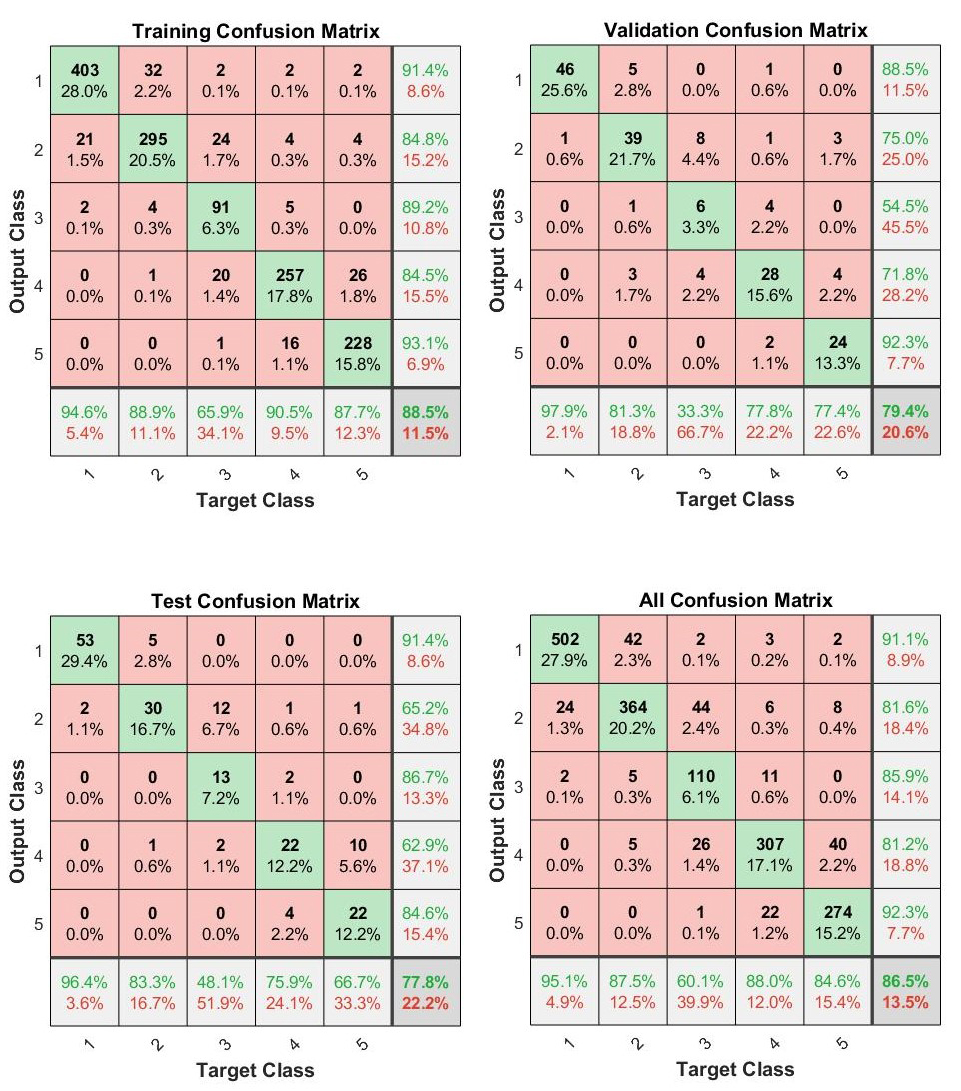
\includegraphics[scale=0.5]{confusion2}
        \caption{Matrice di confusione}
    \end{figure}
    \\Come si evince dalla matrice di test, il risultato è abbastanza migliorato, arrivando ad una precisione del 77\%.
    A questo punto è evidente che, data la complessità del problema, potrebbero essere necessarie soluzioni più avanzate per ottenere una precisione superiore. 
    Si ricorre quindi al classificatore ensemble.
    \subsubsection{Classificatore Ensemble}
    Un classificatore ensemble  è un complesso di reti neurali che lavorano separatamente ma contribuiscono all'ottenimento di un risultato comune.
    Le feature di input vengono date in ingresso a tutte le reti e ognuna di queste restituisce un responso sulla base della sua personale esperienza. Tutti i risultati delle reti vengono poi inviati ad una funzione che ha il compito di decidere il risultato finale.
    Per decidere, si usa semplicemente il principio di maggioranza, il responso che è stato dato da più reti è probabilmente quello corretto.
    Nel nostro caso, sono state addestrate 100 reti neurali, dette classificatori, con 18 input e 25 neuroni nascosti. 
    \begin{figure}[h]
        \centering
        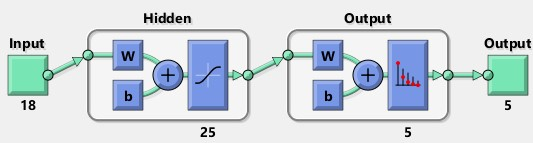
\includegraphics[scale=0.9]{strutturaRete2}
        \caption{Struttura di un classificatore}
    \end{figure}
    \\Selezionando 5 reti che hanno mostrato buone prestazioni, il nostro classificatore ensemble avrà la seguente forma:
    \begin{figure}[h]
        \centering
        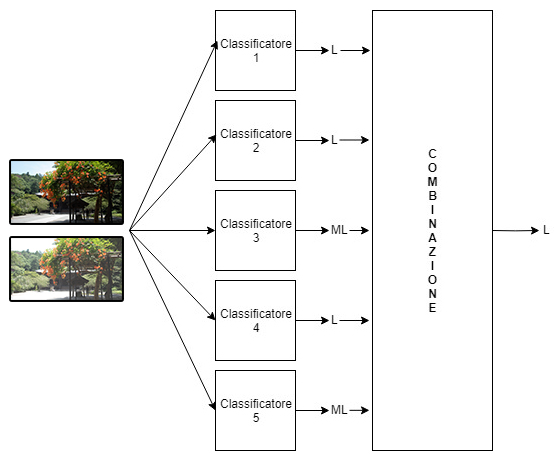
\includegraphics[scale=0.55]{classifier}
        \caption{Classificatore Ensemble}
    \end{figure}
    \newpage
    Sorge un unico problema, cosa fare in una situazione di pareggio? Il criterio adottato è quello di effettuare la media tra i due giudizi vincenti.
    Se tuttavia la media non dovesse ricadere nettamente su un giudizio, ad esempio nel caso di due reti che restituiscono H e due reti che restituiscono M, il giudizio tenderà sempre
    verso il centro (e quindi verso M), poiché è considerata una risposta più plausibile in presenza di indecisione.
    Sia $r$ la matrice contenente i responsi dei 5 classificatori ordinate per riga, la funzione Matlab per stabilire il giudizio finale è:
    \begin{lstlisting}[language=Matlab]
        % Si calcola la somma per colonna 
        total = sum(r);

        % L'indice della colonna associata alla somma maggiore
        % corrisponde al giudizio maggiormente scelto
        maxValue = max(total);
        indexes = find(total == maxValue);

        % Gestione dei pareggi
        if length(indexes) > 1 
            average = mean(indexes)
            if floor(average) ~= average

            if average < 3
                y = ceil(average)
            else
                y = floor(average)
            end
            else 
                y = average;
            end
        else 
            y = indexes;
        end
    \end{lstlisting}
    \newpage
    \subsubsection{Valutazione delle prestazioni del classificatore ensemble}
    Si valuta l'errore commesso dal classificatore ensemble su due dataset. Il primo, sarà l'intero dataset preso in considerazione durante la ricerca.
    Il secondo sarà il risultato dell'unione dei soli sample di test che sono stati usati durante l'addestramento delle singole reti. 
    Di seguito sono riportate le matrici di confusione nei due casi:
    \begin{figure}[h]
        \centering
        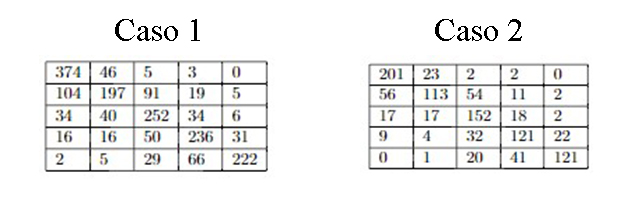
\includegraphics{confusion3}
        \caption{Matrici di confusione}
    \end{figure}
    \\Analizzandole si ottiene una precisione di poco inferiore al 90\%, per la precisione dell'88\% in entrambi i casi. 
    Abbiamo raggiunto una precisione adeguata, considerando che stiamo risolvendo un problema di classificazione a 5 classi e possiamo usare questa rete per effettuare il test.
    \newpage
    \section{Test}
    Si procede quindi sfruttando la rete neurale per capire se, al calare della risoluzione, le differenze percettive tra due immagini continuano ad essere visibili.
    Vengono quindi selezionati 8 campioni significativi dal dataset contenente i confronti tra le immagini e passati alla rete neurale. 
    Dai risultati ottenuti dalla rete neurale, si tracciano dei grafici sull'andamento del giudizio considerandolo come un valore numerico da 1(L) a 5(H):
    \begin{figure}[h]
        \centering
        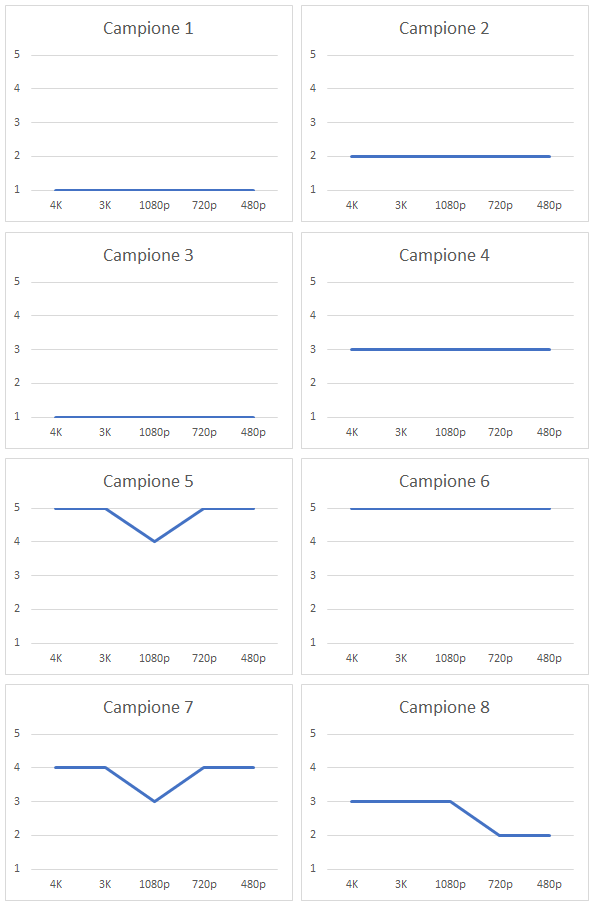
\includegraphics[scale=0.48]{campioni}
        \caption{Test sui campioni}
    \end{figure}

    \newpage
    \section{Conclusioni} 
    Analizzando i risultati ottenuti durante la fase di test risulta evidente che, al calare della risoluzione, 
    le differenze percettive tra due immagini continuano ad essere visibili e tendono leggermente ad accentuarsi.
    Si può quindi dire che queste elaborazioni possono essere fatte in sicurezza anche a 480p. 
    Sfruttando l'esempio del paragrafo 2.3.1, un'elaborazione effettuata su 4K necessita di lavorare su 8.294.400 pixel, mentre su 480p i pixel si riducono a soli 261.120.
    Si ricava immediatamente che il risparmio di tempo derivante da questo abbassamento di risoluzione è di circa il 97\%.
    Questo risultato permetterà di risparmiare tempo e denaro, utilizzando strumenti per l'acquisizione di immagini
    a risoluzioni più basse (e quindi più veloci), riducendo anche il tempo di elaborazione tra le immagini da confrontare.\\
    Il risparmio di tempo consentirà inoltre di effettuare un maggior numero di test su più campioni diversi, aumentando notevolmente la possibilità di individuare falle 
    nei processi produttivi e consentendo agli operatori di porvi prontamente rimedio.
    \newpage
    \section{Ringraziamenti}
    Questa avventura è giunta al termine e non posso non approfittarne per ringraziare tutte le persone che hanno reso speciali questi anni.\\[0.1in]
    Il mio primo ringraziamento va a coloro che mi hanno permesso di intraprendere questo percorso, credendo in me e sostenendomi fin dal primo giorno, i miei genitori, Silvio e Aurora. Grazie per avermi appoggiato in tutte le mie scelte e per non aver mai smesso di essere orgogliosi di me. \\[0.1in]
    A mia sorella Ambra e a mio cognato Giovanni che mi sono sempre stati vicini nonostante la distanza. Grazie per aver reso questi anni meno duri con la vostra presenza e i vostri preziosi consigli.\\[0.1in]
    A mio nonno Vincenzo, alle mie nonne Lina e Gemma e a mia zia Anna, per essere stati un punto di riferimento durante tutti questi anni, accompagnandomi nella crescita e trasmettendomi tutti i vostri valori.\\[0.1in]
    Grazie a mia zia Ornella, per avermi dato la spinta iniziale per affrontare tutte le sfide matematiche che questo percorso aveva in serbo per me.\\[0.1in]
    Ringrazio poi il professor Pistolesi, per il grande aiuto e infinita disponibilità dimostratemi nel periodo passato a redigere la tesi insieme e per avermi trasmesso molte delle competenze che mi saranno fondamentali nella mia futura carriera.\\[0.1in]
    Come non citare Simone, amico di una vita e fratello, onnipresente in tutti i momenti salienti della mia vita. Nel corso degli anni ci siamo fatti tanti film in testa, uno più assurdo dell’altro, ma il vero film è la nostra amicizia e io non avrei potuto scegliere persona migliore con cui girarlo.\\[0.1in]
    Un grazie a Ciccio, per aver reso questi anni più spensierati con le sue idee fuori dagli schemi e la sua infinita simpatia.\\[0.1in]
    Infine, voglio ringraziare tutti i miei colleghi e amici, per non avermi mai lasciato solo nelle difficoltà andando avanti uniti verso la meta e sostenendoci l’un l’altro.\\[0.1in]
    Ne è passato di tempo da quando ho intrapreso questa strada tortuosa e piena di difficoltà, ma guardandomi indietro queste diventano irrilevanti e riaffiorano soltanto tutti i bei momenti che hanno costellato questi preziosi anni, resi indimenticabili da ognuno di voi.\\[0.1in]
    Grazie a tutti!
    \end{document}
